\documentclass[12pt,oneside,final]{siuethesis}
\usepackage{microtype} % (optional) for more beautiful typesetting
\usepackage{graphicx} 
\usepackage{hyperref} %makes links clickable
\hypersetup{colorlinks,citecolor=black,filecolor=black,linkcolor=blue,urlcolor=black} %good for electronic copy
\hypersetup{colorlinks,citecolor=black,filecolor=black,linkcolor=black,urlcolor=black}%required for paper graduate school copy
%\usepackage[alphabetic]{amsrefs} %required if using amsrefs, comment out if using bibtex
\usepackage{fixltx2e}
\usepackage{amsmath}
\usepackage{epsf}
%\usepackage{float}
\usepackage{caption}
\usepackage{subfig}
%\usepackage{subcaption}
\usepackage{listings}
\usepackage{rotating}
\usepackage{tabularx}

\usepackage{multirow}

%% controls numbering of theorems
%% this can be configured to your advisor's taste
\newtheorem{theorem}{Theorem}[chapter] %theorem number resets each chapter
\newtheorem{conclusion}[theorem]{Conclusion}
\newtheorem{condition}[theorem]{Condition}
%% conjectures, corollary, defn, etc. numbered sequentially from beginning of chapters
\newtheorem{conjecture}[theorem]{Conjecture} 
\newtheorem{corollary}[theorem]{Corollary}
\newtheorem{example}[theorem]{Example} 
\newtheorem{lemma}[theorem]{Lemma}
\newtheorem{proposition}[theorem]{Proposition}
\newtheorem{solution}[theorem]{Solution}
\theoremstyle{definition}
\newtheorem{definition}[theorem]{Definition}


\author{Bryan Orabutt}
\title{Design and Analysis of a Mult-Channel Discriminator Integrated Circuit for Use in Nuclear Physics Experiments}

%%\advisor{John Q.\ Faculty} %% or 
\advisor{Dr.}{George L. Engel}
\secondreader{Dr.}{Bradley Noble} %% or \secondreader{Dr.}{Karl Gauss}
\thirdreader{Dr.}{Timothy York}
%\fourthreader{Karl Gauss, Sr.}
%\fifthreader{Karl Gauss, Sr.}
%\secondadvisor{Karl Gauss} %if you haves two advisors (rare) then use this line also and pass the option `twoadvisors' to the class
%\abstracttext{Chairperson: The Honorable Jill Smith} %optional -- you can use this to override the text on the abstract page; the grad school default is built-in
\submitdate{August, 2018} %date the month/year submitted to grad school, use a comma between
\copyrightyear{2016} %optional, but required if copyrighted

%% all of these are optional; defaults are shown
\major{Electrical Engineering} 
\degree{Master of Science} %can be used to specify M.A., etc.
\highestdegree{Master of Science} %used if the author already has another graduate degree
\department{Electrical and Computer Engineering} 
%\departmentname{Department}
%\refname{REFERENCES} 

%\captionsetup{width=0.7\textwidth}

\begin{document}
\maketitle 

\frontmatter %signals single spacing/roman numeral pagination

\copyrightpage %optional


% ^^^^^^^^^^^^^^^^^^^^^
% ABSTRACT
% ^^^^^^^^^^^^^^^^^^^^^

\begin{abstract}

This thesis documents the design, analysis, and simulation of a multi-channel integrated circuit (IC) consisting of 16 channels of constant fraction discrimination for use in Nuclear Physics experiments.  

\end{abstract}


% ^^^^^^^^^^^^^^^^^^^^^^^^^^^^^^^^^^^^^^^
% ACKNOWLEDGEMNTS
% ^^^^^^^^^^^^^^^^^^^^^^^^^^^^^^^^^^^^^^^^


\begin{acknowledgements}

I  would  like  to thank  Dr.  Lee  Sobotka  and  Mr.  Jon  Elson,  department  of  chemistry, 
Washington  University  Saint  Louis,  for  their  help  during  the  various  stages  of  this  project. 
My  special  thanks  to  the  faculty  and  staff  of  ECE  department  for  their  direct  and  indirect 
support without which I simply could not have progressed with my work. 



\end{acknowledgements}

\tableofcontents

\cleardoublepage %cause correct numbering of list of figures

\acknowledgements

\cleardoublepage

\listoffigures %print list of figures page

\cleardoublepage

\listoftables

\mainmatter %signals single spacing/arabic numeral paginations

% ^^^^^^^^^^^^^^^^^^^^^^^^^^^^^^^^^^^^^^^^^^^^^^^^^^^^^^^^^
%  CHAPTER 1
% ^^^^^^^^^^^^^^^^^^^^^^^^^^^^^^^^^^^^^^^^^^^^^^^^^^^^^^^^^

\chapter{INTRODUCTION}  %% chapter titles must be typed in all caps to conform with regulations

This chapter will introduce the reader to the field of radiation monitoring and describe how custom multi-channel integrated circuits is helping to re-shape this field.  The IC described in this thesis is the newest addition to the family of ICs which are being developed by the IC Design Research Laboratory at Southern Illinois University Edwardsville (SIUE in collaboration with researchers from the Nuclear Reactions Group at Washington University (WUSTL).

\section{Research Background}

The Integrated Circuits Design Research Laboratory at SIUE and the Nuclear Reactions Group at WUSTL have been working (since 2001) on a family of multi-channel custom integrated circuits.  The group became interested in developing a family of microchips for use in the detection and measurement of ionizing radiation because: (1) the need for high-density signal processing in the low- and intermediate-energy nuclear physics community is widespread, and (2) no commercial chips were identified that were capable of doing what the researchers wanted, and (3) the scientists deemed it necessary for the experimenter to be in the designer’s seat. The goal is to develop a ‘‘tool box’’ of circuits,
useful for researchers working with radioactive ion beams, which can be composed in different ways to meet the researchers’ evolving needs and desires.

 
The group’s first success was an analog shaped and peak sensing chip with on-board constant-fraction discriminators and
sparsified readout. This chip is designed for use with arrays of Si strip detectors of medium scale (with the number of channels ranging from a few hundred to a few thousand) and is known as Heavy-Ion Nuclear Physics–16 Channel (HINP16C) [1,2]. 

The second chip, christened Pulse Shape Discrimination–8 Channel(PSD8C), was designed to logically complement (in terms of detector types) the HINP16C chip. PSD8C performs pulse shape discrimination (PSD), and thus particle identification, if the time dependence of the light output of the scintillator depends on particle type. Moreover, PSD8C uses almost all the same supporting hardware as the HINP16C chip. Both ICs were fabricated in the ON-Semiconductor (formerly AMI) 0.5 mm n-well process (C5N),available through MOSIS (see \url{www.mosis.com}).

Talk about the block diagram of typical PSD system.

\begin{figure}[htbp!]
	\centering
 	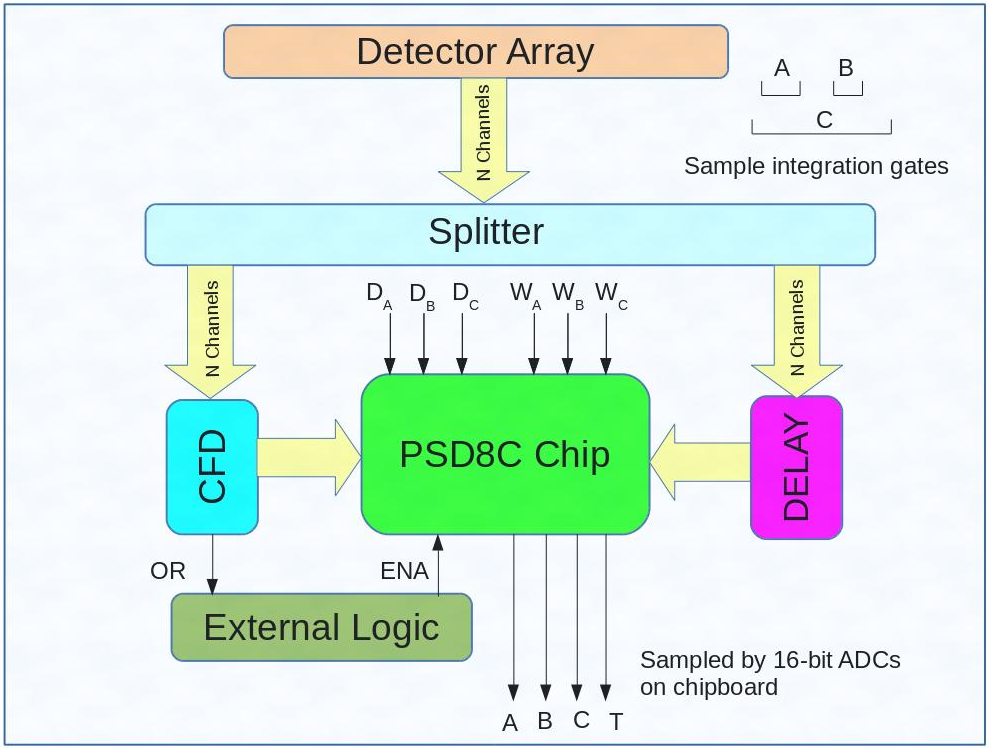
\includegraphics[scale=0.6,keepaspectratio=true]{./ch1_figures/PSD_block.png}
 	\caption{Block diagram of typical PSD system.}
 	\label{FIG:PSD_BLOCK}
\end{figure}


\section{PSD8C IC}

Our PSD8C chip greatly simplifies the pulse-processing electronics needed for large arrays of scintillation detectors. Each channel(see Figure~\ref{FIG:PSD_CHANNEL}) possesses 3 sub-channels. The sub-channels are referred to as A, B, and C. A sub-channel consists of an integrator and a gate generator. External control voltages (DX, WX) determine the gate delay and the gate width. The structure of a single PSD8C sub-channel is illustrated in Figure~\ref{FIG:PSD_SUB_CHANNEL}. Because PSD8C employs (user-controlled) multi-region charge integration, particle identification is incorporated into the basic design. Each channel on the chip also contains a TVC that provides relative time information. The pulse height integrals and the relative time are all stored on capacitors and are either reset, after a user-controlled time, or sequentially read out if acquisition of the event is desired (in a manner similar to that of HINP16C). 

\begin{figure}[htbp!]
	\centering
 	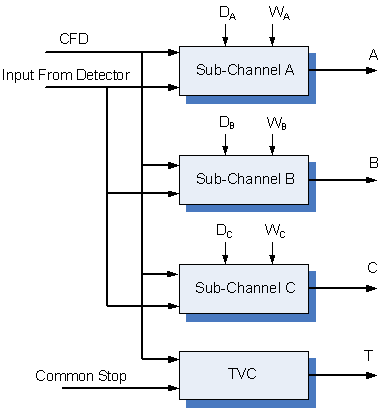
\includegraphics[scale=1.0,keepaspectratio=true]{./ch1_figures/PSD_channel.png}
 	\caption{PSD Channel}
 	\label{FIG:PSD_CHANNEL}
\end{figure}


\begin{figure}[htbp!]
	\centering
 	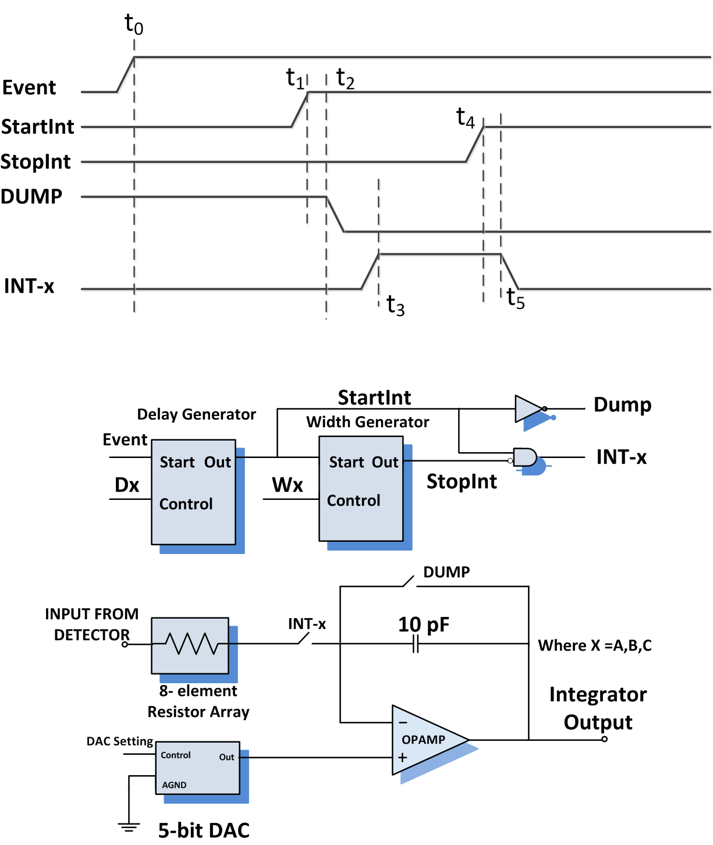
\includegraphics[scale=1.3,keepaspectratio=true]{./ch1_figures/PSD_sub_channel.png}
 	\caption{PSD Sub-channel.}
 	\label{FIG:PSD_SUB_CHANNEL}
\end{figure}

Features of the first generation PSD8C (Rev. 1) chip include:
\begin{itemize}
\item
eight independent channels per IC;
\item
on-chip data sparsification;
\item
each channel automatically resets itself after a user programmable delay time;
\item
three (3) integration regions each with: (a) independent
control of time offset (beginning), (b) width (ending) of the
integration window, and (c) a menu of eight (8) charging rates;
\item
each channel possesses a TVC with two time ranges: 500 ns and 2 ms;
\item
three triggering modes;
\item
fast logical OR-gate and an analog multiplicity output to aid in
trigger decisions;
\item
two power modes to facilitate use with fast and slow detectors
and to thus allow for a more modest power budget for the
latter; 
\item
and CFD circuits are not on-chip so as to provide greater flexibility.
\end{itemize}

PSD8C is described in detail in Refs. []. PSD8C is 2.25 by 5.7 $mm^2$ and is packaged in a 14 by 14 $mm_2$, 128 lead thin quad flat pack. Power consumption is 65 mW (low-bias mode)and 150 mW (high-bias mode). The cost per channel is 25.
A second version (Rev. 2) of PSD8C was submitted for fabrication in May 2010. Rev. 2 attempts to correct several minor
problems. First, the TVC circuit could inadvertently be re-started. In Rev. 2, once the rising edge of the ‘‘common stop’’ signal is detected, the TVC cannot re-start until the channel is reset. Second, undesirable temperature dependence (1 ns/C) in the TVC circuit was identified and traced to the local channel buffer. The buffer was redesigned, and the TVC temperature sensitivity has been greatly reduced (5 ps/C in the 500 ns mode, 40 ps/C in the 2 ms mode). Third, some TVC crosstalk issues were identified and remedied. Fourth, additional shielding was added to the integrator circuits. Finally, at the system level, the chip-boards (printed-circuit boards) were redesigned to include on-board ADCs (one for each of the chip’s analog output pulse trains).

(Still need to talk about enhancements that were made on PSD4)


\section{Need for an Integrated Circuit}

While not including the timing circuits on PSD made it more flexible, those circuits are needed.  Currently, a large complex board with many ICs produce the timing signals required by the PSD chip. This thesis describes the design of multi-channel integrated circuit which can generate the timing signals for a pair of PSD chips.

\begin{figure}[htbp!]
	\centering
 	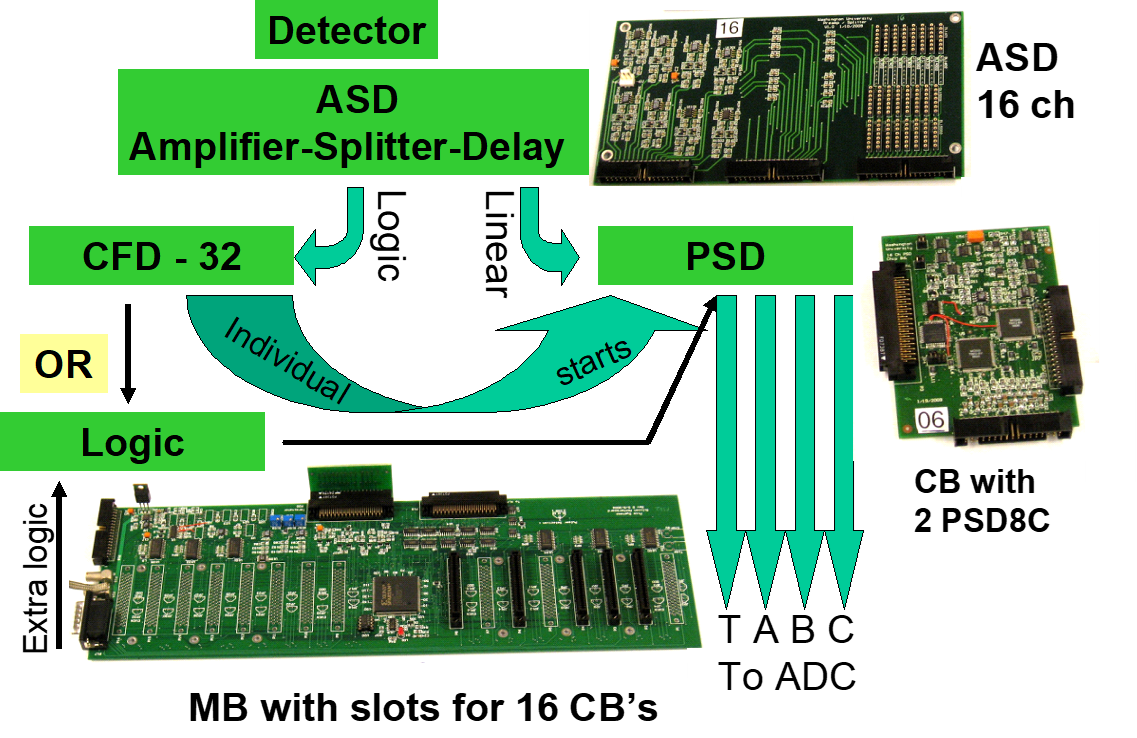
\includegraphics[scale=0.9,keepaspectratio=true]{./ch1_figures/PSD_system.png}
 	\caption{PSD system using board-level CFD electronics}
 	\label{FIG:PSD_SYSTEM}
\end{figure}



\section{Sample Applications}

To focus the reader’s attention on what would be possible with the PSD chip complemented by the CFD chip described in this tehses, consider a highly granular discrete element array for neutron detection using the recently developed inorganic [9] and plastic [11] scintillators with PSD. Such a large array would open the n-rich side up to the kind of high-precision work the Washington University group has done on the p-rich side. (The existing work on the neutron-rich side, done at high energy and with detectors such as MONA-LISA [12], while providing provocative data on such cases as 16Be [13] and 26O [14], sufferer for poor statistics and, compared to the proton-rich side, poor resolution.) An array to be deployed at low (reaccelerated beam) energies with thousands of optically isolated PSD elements made from the new generation of plastics, would revolutionize the study of multiple n-decay from what are generally high-isospin states. (The problem of detector-to-detector scattering cross-talk can also be improved with discrete pixilated – rather than using large bars – by corrugating the detectors in the same way as the conventional discrete array DEMON has [15].  

While we are enamored with the above idea, it is premature to propose such an array before the ground-work for scalable timing electronics, as we describe in this thesis, is successfully completed. (In fact the coupling of the scintillator – from Eljen – to the new blue sensitive SiPMs – from SensL – is simple compared to the development of the scalable electronics.) To this end however, we plan to develop a circuit board using the PSD and CFD chips to process signals from the new generation of PSD-capable plastic scintillators [11]. 

The CFD chip described herein with its programmable Nowlin cirucit will allow the WUSTL Nuclear Rewactions Gropup to work with variety of scintillators (LaBr:Ce to CsI:Tl or :Na to standard plastics and, for what might be the most interesting untapped opportunity, the new class of PSD capable plastics [11)].  


\section{Object and Scope of Work} 

% ^^^^^^^^^^^^^^^^^^^^^^^^^^^^^^^^^^^^^^^^^^^^^^^^^^^^^^^^^
%  CHAPTER 2
% ^^^^^^^^^^^^^^^^^^^^^^^^^^^^^^^^^^^^^^^^^^^^^^^^^^^^^^^^^


\chapter{SYSTEM ARCHITECTURE}

This chapter will attempt to describe the CFD16C integrated circuit at the system-level.  We will start with a detailed list of system requirements and then will describe the high-level architecture of the IC.

\section{System Specifications}
The success of our group over the past 20 years lies in the fact that in the close working relationship that the IC Design Research Laboratory at Southern Illinois University Edwardsville (SIUE) has had with the Nuclear Reactions Group at Washington University in St. Louis(WUSTL) led by Dr. Lee Sobotka.  The IC group here at SIUE and the Nuclear Reactions Group at WUSTL, after lengthy discussions, drafted the following specifications for the IC described here in this thesis.

\begin{itemize}
\item
The IC should support 16 detectors.
\item
It should support analog pulses of both polarities (relative to analog signal ground).
\item
It should accommodate analog exponentially shaped pulses with risetime constants ranging from 3 nsec to 100 nsec.
\item
It exhibit "excellent" walk and jitter characteristics for input pulse amplitudes ranging from 20 mV to 2 V. The adjective "excellent" will be quantified in a later chapter of this thesis.
\item
Pulse repetition rates up to 1 KHz must be accommodated.
\item
The discriminator in each of the 16 channels should be of the constant fraction type (CFD). In CFD discriminators an attenuated version of the input is subtracted from a delayed version of input waveform and the time at which the difference between the two is equal to zero is used to mark the pulse arrival time. This results in output timing signals independent of pulse amplitude.
\item
Each channel should have a leading-edge threshold.
\item
While the chip must support signals with risetime constants ranging from 3 nsec to 100 nsec, performance will be optimized for the shorter time constants. 
\item
The output pulse width from a channel should be programmable.
\item
The IC should operate from a single 3.3 Volt supply.
\item
Power consumption of the 16 channel IC should not exceed 350 mW \emph{i.e.} 20 mW per channel with 30 mW budgeted for the circuits common to all channels. 
\item
The IC is not to occupy an area greater than roughly 2 mm x 3 mm.  The chip should be packaged in a 64-pin plastic package.  

\end{itemize} 

\section{Features}

\section{System-Level Description}

\section{Chip Pinout}

% ^^^^^^^^^^^^^^^^^^^^^^^^^^^^^^^^^^^^^^^^^^^^^^^^^^^^^^^^^
%  CHAPTER 3
% ^^^^^^^^^^^^^^^^^^^^^^^^^^^^^^^^^^^^^^^^^^^^^^^^^^^^^^^^^


\chapter{ELECTRICAL LEVEL DESIGN}

\section{Fabrication Process}

The IC described in this thesis will be fabricated in the AMS-AG 0.35 micron NWELL process.  The process supports two poly and 4 metal layers. Double poly capacitors, BJTs, and a high-resistance layer are all available to the designer. NFET device properties are given in Table~\ref{TBL:NMOS_PARMS} while PFET device properties are availabe in Table~\ref{TBL:PMOS_PARMS}.

% NFET device properties

\begin{table} [htbp!]
\begin{center}
\begin{tabular}{| l | c | c |}
\hline 
Threshold Voltage & $V_{TN}$ & 0.5 V \\ 
\hline 
Transconductance Parameter & $K_{PN}$  &  170 $\frac{\mu A}{V^2}$ \\ 
\hline 
Bulk Modulation Factor & $\gamma_{N}$  &  0.6 $V^{\frac{1}{2}}$ \\ 
\hline 
Early Voltage per Unit Length & $V_{EN}$  &  21.1 $\frac{V}{\mu m}$ \\ 
\hline 
Gate Oxide Thickness & $t_{ox}$  &  7.6 nm \\ 
\hline 
Gate Oxide Capacitance per Unit Area & $C_{ox}$  & 4.5 $\frac{fF}{\mu m^2}$ \\ 
\hline 
Threshold Voltage Matching Coefficient & $A_{VTN}$  &  9.4 mV $\cdot$ $\mu m$ \\ 
\hline 
Transconductance Matching Coefficient & $A_{KPN}$  &  0.7 \% $\cdot$ $\mu m$ \\ 
\hline 
\end{tabular} 
\end{center}
\label{TBL:NMOS_PARMS}
\caption{NMOS Parameters}
\end{table}

% PFET device properties
 
\begin{table} [htbp!]
\begin{center}
\begin{tabular}{| l | c | c |}
\hline 
Threshold Voltage & $V_{TP}$ & -0.7 V \\ 
\hline 
Transconductance Parameter & $K_{PP}$  &  60 $\frac{\mu A}{V^2}$ \\ 
\hline 
Bulk Modulation Factor & $\gamma_{P}$  &  0.4 $V^{\frac{1}{2}}$ \\ 
\hline 
Early Voltage per Unit Length & $V_{EP}$  &  17.7 $\frac{V}{\mu m}$ \\ 
\hline 
Gate Oxide Thickness & $t_{ox}$  &  7.6 nm \\ 
\hline 
Gate Oxide Capacitance per Unit Area & $C_{ox}$  &  4.5 $\frac{fF}{\mu m^2}$ \\ 
\hline 
Threshold Voltage Matching Coefficient & $A_{VTP}$  &  14.5 mV $\cdot$ $\mu m$ \\ 
\hline 
Transconductance Matching Coefficient & $A_{KPP}$  &  1.0 \% $\cdot$ $\mu m$ \\ 
\hline 
\end{tabular} 
\end{center}
\caption{PMOS Parameters}
\label{TBL:PMOS_PARMS}
\end{table}

% DESCRIPTION OF COMMON CHANNEL

\section{Common Channel}

\subsection{Configuration registers}

\subsection{Power on reset circuit}

\subsection{Signal ground generator}

\subsection{Bandgap voltage reference}

\subsection{PTAT current reference}

\subsection{Zero-tempco current reference}

\subsection{Lockout DAC}

\subsection{Multiplicity output buffer}


% DESCRIPTION OF SIGNAL CHANNEL

\section{Signal Channel}

\subsection{Programmable Nowlin circuit}

\subsection{Leading-edge detector}

\subsection{Zero-cross detector}


\subsection{Output one-shot with lockout features}



% ^^^^^^^^^^^^^^^^^^^^^^^^^^^^^^^^^^^^^^^^^^^^^^^^^^^^^^^^^
%  CHAPTER 4
% ^^^^^^^^^^^^^^^^^^^^^^^^^^^^^^^^^^^^^^^^^^^^^^^^^^^^^^^^^


\chapter{SIMULATION RESULTS}

\section{Verification of Circuits in Common Channel}

\section{Walk Characteristics of CFD Circuitt}

\section{Jitter Performance}

\section{Verification of One-Shot}

\section{Performance Characterization of DAC}

\section{Chip-Level Verification}


% ^^^^^^^^^^^^^^^^^^^^^^^^^^^^^^^^^^^^^^^^^^^^^^^^^^^^^^^^^
%  CHAPTER 5
% ^^^^^^^^^^^^^^^^^^^^^^^^^^^^^^^^^^^^^^^^^^^^^^^^^^^^^^^^^


\chapter{SUMMARY, COMCLUSIONS, AND FUTURE WORK}

\section{Summary}


\section{Conclusions}

\section{Future Work}

\references %single spacing / arabic numeral paginations, adds "REFERENCES" to table of contents

%%%% for bibtex

%If you want to use bibtex  use the following lines, where your .bib file is called 'yourbib.bib'

\bibliographystyle{apalike}
\bibliography{./Orabutt_Thesis.bib}

% If you have only a single appendix, do it this way.

\multipleappendices
\lstset{
         language=C,
         basicstyle=\scriptsize\ttfamily,
         emptylines=0, 
         lineskip=1pt,
         %numbers=left,            
         numberstyle=\tiny,         
         stepnumber=2,              
         numbersep=5pt,             
         tabsize=3,                
         extendedchars=true,       
         breaklines=true,            
         commentstyle=\color{blue},
         keywordstyle=\color{red},
            frame=b,         
 %        keywordstyle=[1]\textbf,    
 %        keywordstyle=[2]\textbf,    
 %        keywordstyle=[3]\textbf,  
 %        keywordstyle=[4]\textbf,   \
         stringstyle=\scriptsize\color{green}\ttfamily, 
         showspaces=false,         
         showtabs=false,            
%         xleftmargin=17pt,
%         framexleftmargin=17pt,
%         framexrightmargin=5pt,
%         framexbottommargin=4pt,
         %backgroundcolor=\color{lightgray},
         showstringspaces=false           
 }


\end{document}
